\documentclass[aspectratio=169]{beamer}
% \setbeameroption{show notes on second screen}

\usepackage{lmodern}
\usepackage{array}
\usepackage{romannum}
\usepackage{amsmath}
\usepackage{soul}
\usepackage[overridenote, duration=20]{pdfpc}

\beamertemplatenavigationsymbolsempty
\setbeamertemplate{footline}[frame number]{}
\setbeamertemplate{caption}{\raggedright\insertcaption\par}
\newcommand{\diff}{\operatorname{d}}

\newcommand{\overbar}[1]{\mkern 1.5mu\overline{\mkern-1.5mu#1\mkern-1.5mu}\mkern 1.5mu}
\title{Barycenter's exsitence in the Wasserstein space\\ over a proper space}
\author{Jianyu MA}
\date{\today}

\begin{document}

\frame{\titlepage}

\section{Existence and counter-examples}
\begin{frame}
	\frametitle{Barycenter in a metric space $(E,d)$}
	\setbeamercovered{
		% still covered={\opaqueness<1->{8}},
		again covered={\opaqueness<2->{15}}
	}
	\begin{definition}
		\onslide<1>{
			Let $\mu$ be a probability measure on $(E,d)$,
			$z \in E$ is
			a \emph{\textcolor{cyan}{barycenter} of $\mu$} if
		}
		\[
			z \in \arg\min_{x \in E} \int_{E} d(x,y)^2 \diff \mu(y)
			\onslide<1>{.}
		\]
	\end{definition}
	\begin{overlayarea}{\textwidth}{1.5cm}
		\begin{description}
			\item<2 | only@2>[Intuition] $ \displaystyle E = \mathbb{R} \implies z = \int_{\mathbb{R}} y \diff \mu(y) $
			\\[0.2cm]
			In Statistics, $z$ is a mean of $\mu$.
			\item<3 | only@3>[Unknown] \textcolor{purple}{Existence} and uniqueness
		\end{description}
	\end{overlayarea}
\end{frame}

\begin{frame}
	\frametitle{Barycenter's existence in $(E,d)$}
	\setbeamercovered{
		still covered={\opaqueness<1>{15}},
		% again covered={\opaqueness<1>{10}}
	}
	\onslide<1,2>{When $(E,d)$ is a}
	\begin{description}
		\item<1,3>[proper space:] \textcolor{teal}{closed + bounded = compact}%
		\onslide<1>{,\\[0.1cm]
			barycenter always exists.}
		\item<2,3>[length space:] \textcolor{teal}{distance = inf of length of curves}%
		\onslide<2>{,\\[0.1cm]
			$z$ a barycenter of $\frac{1}{2}\delta_x + \frac{1}{2}\delta_y \Longleftrightarrow
				d(x,z)=d(z,y) = \frac{1}{2}d(x,y)$.}
	\end{description}
	% \setbeamercovered{invisible}
	\vfill
	\onslide<3>{
		\begin{theorem}[Hopf-Rinow]
			Locally compact + complete + length space $\implies$ proper
		\end{theorem}
	}
\end{frame}

\begin{frame}[t]
	\frametitle{Counter-examples of barycenter's existence}
	\only<1>{
		\begin{example}[Locally compact complete \textcolor{gray}{\st{length}} space]
			$\mathbb{R}$ with $d(x,y) = \phi(|x-y|)$, measure
			$\mu = \frac{1}{2} \delta_{1} + \frac{1}{2} \delta_{-1}$:
			\begin{figure}[h]
				\centering
				\begin{minipage}{.49\textwidth}
					\centering
					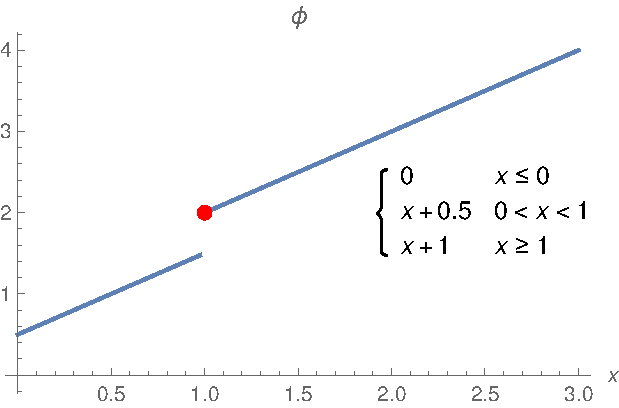
\includegraphics[height=.48\linewidth]{Chapters/example_phi.pdf}
					\caption{$ \displaystyle d(x,y):=\phi(|x-y|)$}
				\end{minipage}
				\begin{minipage}{.49\textwidth}
					\centering
					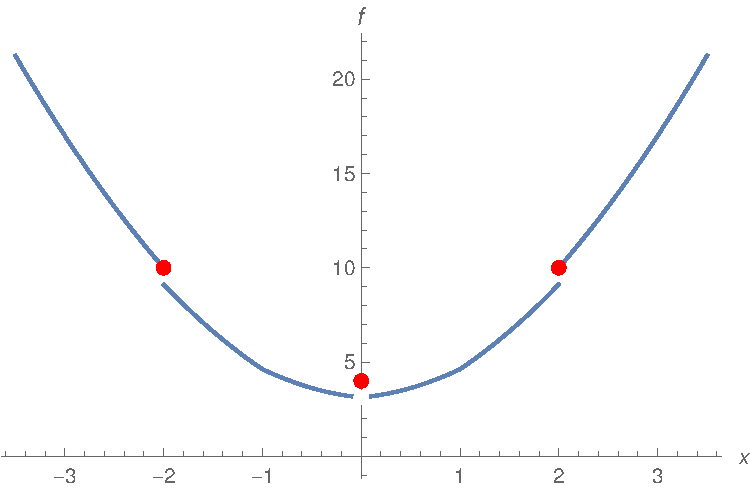
\includegraphics[height=.50\linewidth]{Chapters/example_f.pdf}
					\caption{$\displaystyle f(x) :=\int_{\mathbb{R}} d^2(x,y) \diff \mu(y)$}
				\end{minipage}
			\end{figure}
		\end{example}
	}
	\only<2>{
		\begin{example}[Locally compact \textcolor{gray}{\st{complete}} length space]
			The unit disk with center removed.
			% $\mathbb{D} \backslash \{0,0\}$
			\\[0.3in]
			\textcolor{gray}{
				No barycenter of
				\begin{enumerate}
					\item uniform measure
					\item $\frac{1}{2}\delta_x + \frac{1}{2}\delta_{-x}$
				\end{enumerate}
			}
		\end{example}
	}

	\only<3>{
		\begin{example}[\textcolor{gray}{\st{Locally compact}} complete length space]
			Infinite dimensional ellipsoid with axes of decreasing length $c_n := \frac{n+1}{2n}$,
			\[
				E := \left\{ \left( x _ { 1 } , x _ { 2 } , \ldots \right) \in \ell^2 \quad
				\left| \quad \sum _ { n = 1}^{\infty}
				\frac { x _ { n } ^ { 2 } } { c _ { n } ^ { 2 } } = 1 \right. \right\}.
			\]
			$E$ is a smooth Hilbert Riemannian submanifold of $\ell^2$.
		\end{example}
	}
\end{frame}

\section{Wasserstein space}
\begin{frame}
	\frametitle{Wasserstein space $(\mathcal{W}(E), W)$ of probability measures}
	% \setbeamercovered{transparent}
	\setbeamercovered{
		still covered={\opaqueness<1->{8}},
		again covered={\opaqueness<1>{50}}
	}
	Assume $(E,d)$ is
	\textcolor{teal}{complete and separable}
	\onslide<1>{
		\[
			\mathcal{W}(E) = \left\{ \mu
			\, \left| \,
			\int_{E} d(x_0, y)^2 \diff \mu (y) < + \infty \right. \right\}
		\]
	}
	\onslide<2>{
		\textcolor{gray}{
			\begin{align*}
				\textcolor{black}{W ( \mu , \nu )}^2
				 & = \inf \left\{
				\textcolor{black}{\int _ { E \times E} d ( x , y ) ^ 2 \diff \pi ( x , y )}
				,\quad \pi \text{ has marginals } \mu \text{ and } \nu \right\}
				\\[0.5cm]
				 & = \inf \left\{  \textcolor{black}{\mathbb{ E } d ( X , Y ) ^2}
				, \quad \operatorname { law } ( X ) = \mu , \quad \operatorname { law } ( Y ) = \nu \right\}
			\end{align*}
		}
	}
	\onslide<3>{
		\textcolor{gray}{Example:}
		$\displaystyle W(\delta_{x_0} , \mu)^2 = \int_{E} d(x_0, y)^2 \diff \mu(y)
			,\quad W(\delta_x, \delta_y)=d(x,y) $
	}
\end{frame}

\begin{frame}
	\frametitle{Details of Wasserstein metric $W$}
	\setbeamercovered{
		still covered={\opaqueness<1->{0}},
		again covered={\opaqueness<1>{35}}
	}
	\begin{theorem}[Existence of an optimal coupling]
		% Let $(E,d)$ be a Polish space.\\
		\onslide<1>{
			There exists an
			\textcolor{cyan}{optimal coupling}
			% $(X, Y)$ with $\operatorname { law } ( X ) = \mu$ and $\operatorname { law } ( Y ) = \nu$ such that
			$\pi$ of $\mu$ and $\nu$:}
		\[
			W(\mu, \nu)^2 =
			% \mathbb{ E } d ( X , Y ) ^2.
			\int _ { E \times E} d ( x , y ) ^ 2 \diff \pi ( x , y )
			\onslide<1>{.}
		\]
		\onslide<1>{
			Moreover, we call $(X, Y)$ an
			\textcolor{cyan}{optimal coupling} if $\operatorname{law}(X,Y) = \pi$.
		}
	\end{theorem}
	{\small \textcolor{gray}{proof} \;}
	\pause
	by \textcolor{purple}{weak convergence}:
	\begin{enumerate}
		\item the set of all couplings is tight
		\item $\displaystyle f \text{ conti.} \implies \pi \mapsto
			      \int f \diff \pi \text{ lower semi-conti.}$
	\end{enumerate}
\end{frame}

\begin{frame}
	\frametitle{Properties of Wasserstein space $\mathcal{W}(E)$}
	\setbeamercovered{
		again covered={\opaqueness<1->{8}}
	}
	% Basic facts of $(\mathcal{W}(E), W)$:
	\begin{enumerate}
		\item<1> $\mathcal{W}(E)$ is complete and separable\\[0.2cm]
		\item $(E,d)$ is geodesic $\implies$ $\mathcal{W}(E)$ is a geodesic\\[0.2cm]
		      \item<1> $\mathcal{W}(E)$ is locally compact $\implies$ $E$ and $\mathcal{W}(E)$ are compact
	\end{enumerate}
	\setbeamercovered{invisible}
	\pause
	\begin{columns}
		\column{0.5\textwidth}
		\begin{example}[Barycenter in $\mathcal{W}(\mathbb{S}^2)$]
			Midpoint between two uniform measures on
			the mainland shapes of China and France.
		\end{example}
		\column{0.5\textwidth}
		\begin{center}
			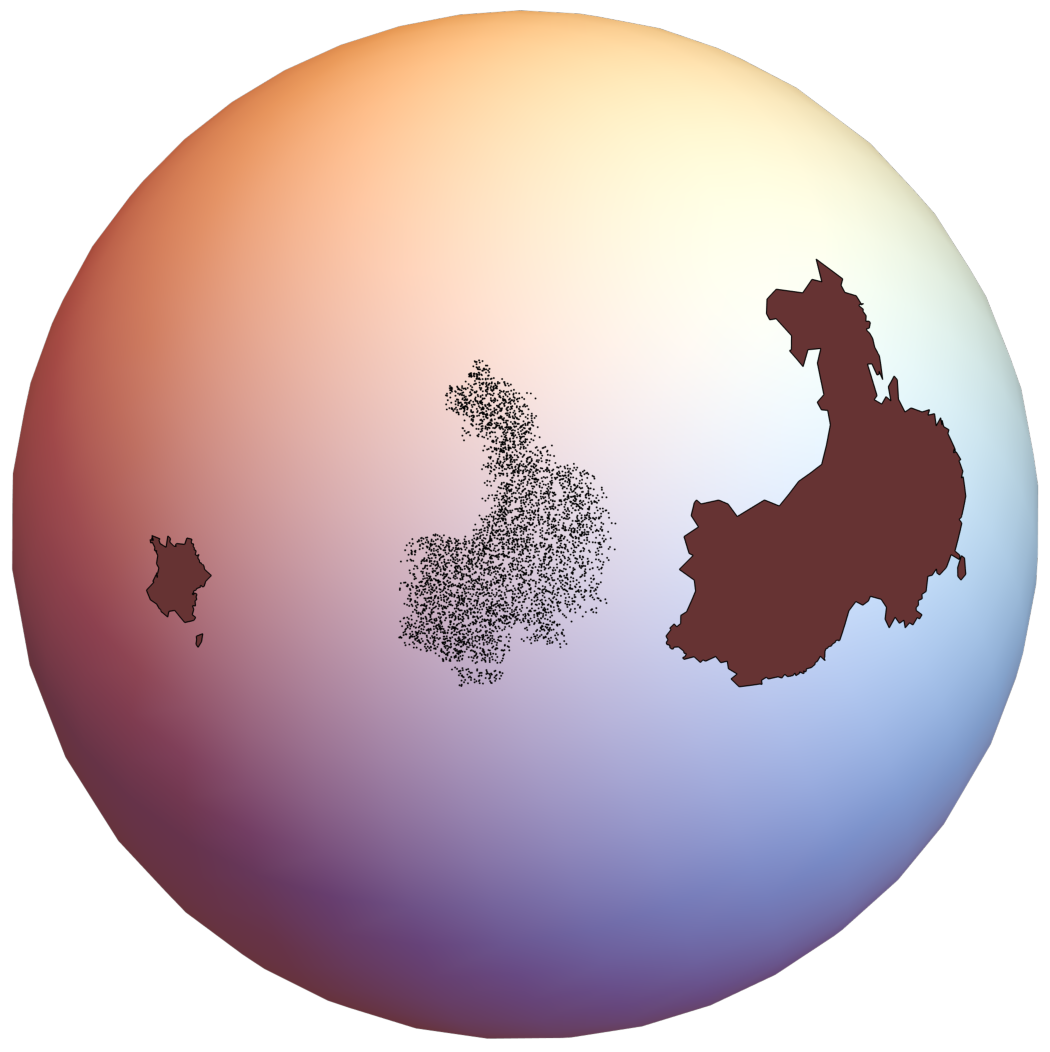
\includegraphics[width=0.5\linewidth]{Chapters/OPT_sphere.pdf}
		\end{center}
	\end{columns}
\end{frame}

\begin{frame}
	\frametitle{Barycenter's existence for measure
		$ \displaystyle \sum_{i=1}^n \lambda_i \delta_{\mu_i}$ on $\mathcal{W}(E)$}
	% \setbeamercovered{transparent}
	\onslide<1>{
		Assume $(E,d)$ proper.
		Pick $(X,X_1,\ldots,X_n)$ s.t.\@}
	% $\operatorname{law}(X) = \mu$, $\operatorname{law}(X_i) = \mu_i$ and
	\onslide<1>{
		$W(\mu, \mu_i)^2 = \mathbb{E} d(X, X_i)^2$
	}
	\onslide<1>{, then
	}
	% \onslide<1,3,5>{
	\begin{equation}
		\label{equa:barycenter_selection}
		\sum_{i=1}^n \lambda_i W(\mu, \mu_i)^2 = \mathbb{E} \sum_{i=1}^n \lambda_i d(X, X_i)^2
		\geq \mathbb{E} f(X_1, \ldots, X_n)
		\onslide<1>{,}
	\end{equation}
	% }
	\onslide<1>{
		where }
	\onslide<1-4>{
		$ \displaystyle f(x_1, \ldots, x_n) = \min_{x}
			\sum_{i=1}^n \lambda_i d(x, x_i)^2
			% \min_{x} W^2 (\delta_x, \sum_{i=1}^n \lambda_i \delta_{x_i})
		$ \onslide<1>{.}
		\\[0.3cm]
		\setbeamercovered{invisible}
		\pause
		\textcolor{red}{Claim: $f$ is continuous.}
		$\implies$ existences of
	}
	\begin{enumerate}
		\item $\min \mathbb{E} f(X_1, \ldots, X_n)$ \textcolor{gray}{over all possible $X_i$}
		      \pause
		\item \textcolor{gray}{a measurable
			      \textcolor{black}{selection $B$} from \textcolor{black}{$(x_1,\ldots,x_n)$} to
			      \textcolor{black}{barycenters of $\sum_{i=1}^n \lambda_i \delta_{x_i}$}
			      on $E$}\\
		      \onslide<4>{
			      $\implies$ \emph{\textcolor{gray}{eq.\@ (\ref{equa:barycenter_selection})}} achieves an equality.
		      }
	\end{enumerate}
	\setbeamercovered{invisible}
	\onslide<5>{
		Finally, barycenter \textcolor{blue}{$\bar{\mu} := B_{\#} \gamma$}, where $\gamma$
		is the law of an optimal $(X_1, \ldots, X_n)$.
	}
\end{frame}

\begin{frame}
	\frametitle{Barycenter's existence for any measure $\mathbb{P}$ on $\mathcal{W}(E)$}
	\begin{block}{Consistency of barycenters in $\mathcal{W}(E)$}
		Let $\mu_j$ be a barycenter of $\mathbb{P}_j$.\\
		If $\mathbb{P}_j \rightarrow \mathbb{P}$,
		then $\mu_j$ has a subsequence converging to a barycenter $\mu$ of $\mathbb{P}$.
	\end{block}

	\vfill
	\textcolor{gray}{Application:}\\[0.2cm]

	$\sum_{i=1}^n \lambda_i \delta_{\mu_j}$ is dense in $\mathcal{W}(E)$ $\implies$ Barycenter's existence.
\end{frame}

\section{Ending}

\begin{frame}
	\frametitle{The last part of my internship}
	Assume $E$ is a \textcolor{teal}{complete Riemannian manifold}.

	For barycenters in $\mathcal{W}(E)$, we
	\only<1>{prove}\only<2->{study}
	their \\[0.3cm]
	\begin{overlayarea}{\textwidth}{1.5cm}
		\only<1>{
			\textcolor{beamer@blendedblue}{Uniqueness}
			\begin{enumerate}
				\item $(X,Y)$ optimal coupling $\implies Y = T(X)$
				\item $W(\lambda_1 \, \mu_1 + \lambda_2 \, \mu_2, \nu)^2
					      \leq \lambda_1 \, W(\mu_1, \nu)^2 + \lambda_2 \, W(\mu_2, \nu)^2$
				\item
				      \textcolor{beamer@blendedblue}{1} +
				      \textcolor{beamer@blendedblue}{2} $\implies$
				      $W(\cdot, \nu)^2$ is strictly convex
			\end{enumerate}
		}
		\only<2->{
			\textcolor{beamer@blendedblue}{Absolute Continuity}\\
		}
		\only<2,3>{
			Analysis of \textcolor{purple}{$c$-convex functions}
			\textcolor{gray}{\textsuperscript{[McCann, 2001]}},}
		\only<2>{examples:\\
			\begin{enumerate}
				\item $x \mapsto d(x, y)^2$
				\item $\displaystyle x_1 \mapsto \frac{1}{\lambda_1}
					\min_{x} \sum_{i=1}^n \lambda_i d(x, x_i)^2$
				\item Assume $\mu, \nu$ are absolutely continuous and have compact supports,\\
				      $(X,Y)$ optimal coupling $\implies Y = \exp(-\nabla \textcolor{blue}{\varphi}) \circ X$
			\end{enumerate}
		}%
		\only<3>{properties:\\
			\begin{enumerate}
				\item locally Lipschitz
				\item admit Hessian almost everywhere
			\end{enumerate}
		}
		\only<4>{
			\begin{enumerate}
				\item Assume $\mu_i$ have compact supports and $\mu_1$ absolutely continuous, then\\
				the unique barycenter	$\sum_{i=1}^n \lambda_i \delta_{\mu_i}$ is absolutely continuous.
				\item The general case is not fully understood.
			\end{enumerate}
		}
	\end{overlayarea}
\end{frame}
\end{document}
